\part{Part 4: Applications}

\graphicspath{ {./Pictures/} }
\chapterimage{chapter_head_2.pdf} % Chapter heading image

\chapter{Introduction}
\section{Gmsh}
\section{SU2}
\section{Paraview}

\chapter{Inviscid NACA 0012}
%++++++++++++++++++++++++++++++++++++++++++++++++++++++++++++++
\section{Problem Description}
In this tutorial, we are going to explain how to simulate inviscid flow around an NACA0012 airfoil. Since the flow is assumed to be inviscid, we apply Euler equation for flow modeling. Please note that at high Reynolds numbers, the flow could be assumed to be inviscid, since viscosity term in Navier-Stokes equations becomes negligible. For this example, the flow specifications are provided as follows:
\begin{itemize}
    \item Pressure = 101,325 Pa
    \item Temperature = 273 K
    \item Mach number = 0.8
    \item Angle of attack = 1.25 degree
\end{itemize}
The tutorial has two parts: Flow Solution and Post-Processing. In the first part, we explain how to manage prerequisite files and settings, and how to run the CFD simulation using SU2. In the second part, we explain how to use Paraview software to visualize data obtained form SU2.
%++++++++++++++++++++++++++++++++++++++++++++++++++++++++++++++
\section{Flow solution}
To run the simulation, the SU2 needs two essential files: configuration file (.cfg) and mesh file (.su2). In this example, the following files are located in \textit{01Quickstart} folder:
\begin{enumerate}
\item \textit{inv\_NACA0012}.cfg as a configuration file.
\item \textit{mesh\_NACA0012\_inv}.su2 as a mesh file.
\end{enumerate}
The next step is to copy these two files in directory of SU2, where the execution and script files are located there. To run this simulation, open the command line terminal and enter the following commands:
\begin{table}[htbp]
    \centering
    \begin{tabular}{|l|l|}
    \hline
    Windows     & \begin{tabular}{c} \$ cd "where you saved the package" \\ \$ SU2\_CFD.exe inv\_NACA0012.cfg \end{tabular}
    \\
    \hline
    OSX     & \begin{tabular}{c} \$ cd "where you saved the package" \\ \$ SU2\_CFD.exe inv\_NACA0012.cfg \end{tabular}
    \\
    \hline
    \end{tabular}
\end{table}

The SU2 solver will commence calculation and print out the residuals at every iteration until the specified convergence criteria is achieved. After calculations are done, the following output files should be generated and saved in the SU2 folder:
\begin{itemize}
    \item \textit{flow}.vtk: contains the full volume flow solution.
    \item \textit{force\_breakdown}.dat: contains forces and moment on the airfoil.
    \item \textit{history}.vtk: contains convergence history of calculations.
    \item \textit{restart\_flow}.dat: for restarting simulation.
    \item \textit{surface\_flow}.vtk: flow solution on the surface of the airfoil.
    \item \textit{surface\_flow}.csv: comma separated values of flow solution on the airfoil (If you want to plot data in another software, like Microsoft Excel, you can use this file).
\end{itemize}
Please keep in mind that every time you run SU2, the output data will be overwritten. Hence, before launching new simulation, you could make a new folder and transfer your data from previous simulation to this folder.
%++++++++++++++++++++++++++++++++++++++++++++++++++++++++++++++
\section{Post-processing}
In this section, we explain how to use Paraview to visualize CFD data for this example. First of all, install Paraview (this tutorial uses Paraview 3.12.0) if you do not have it on your computer. Otherwise, take following steps for visualization:
%--------------------------------------------------------------
\subsection{Load Solution File:}
Launch Paraview. Go to \textbf{File} $\rightarrow$ \textbf{Open}, and then select \textit{flow}.vtk file. On the left-hand side of Paraview window you will see the file appears under \textbf{builtin} in \textbf{Pipeline Browser}. Now press \textbf{Apply} button in \textbf{Properties} tab, just right under the  \textbf{Pipeline Browser}. After taking these steps, your file is loaded by software and is ready to visualize (Fig.\ref{fig:load}).
\begin{figure}[htbp]
    \centering
    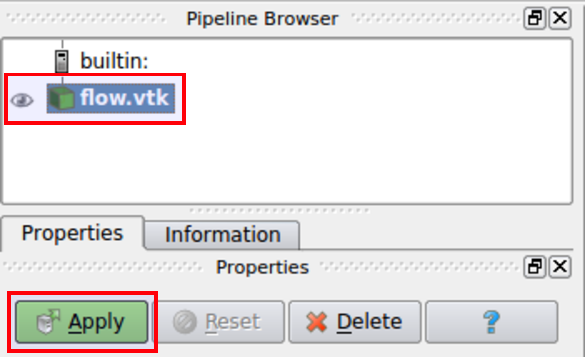
\includegraphics[width=0.4\textwidth]{tut01/loadvtkfile.pdf}
    \caption{Loading .vtk file in the \textbf{Pipeline Browser}.}
    \label{fig:load}
\end{figure}
%--------------------------------------------------------------
\subsection{Visualize Mesh Domain}
In order to view mesh, according to Fig.\ref{fig:wireframe}, select \textit{Solid Color} with \textit{Wireframe} in the toolbar. Then, you can zoom in to see mesh around the airfoil like Fig.\ref{fig:mesh}. As you can see, the mesh around the NACA0012 is unstructured, and the grids are clustered around the leading and trailing edges of the airfoil.
\begin{figure}[htbp]
    \centering
    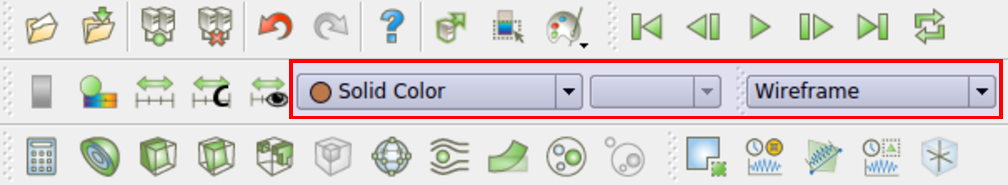
\includegraphics[width=0.6\textwidth]{tut01/wireframe.pdf}
    \caption{How to display mesh in computational domain.}
    \label{fig:wireframe}
\end{figure}
\begin{figure}[htbp]
    \centering
    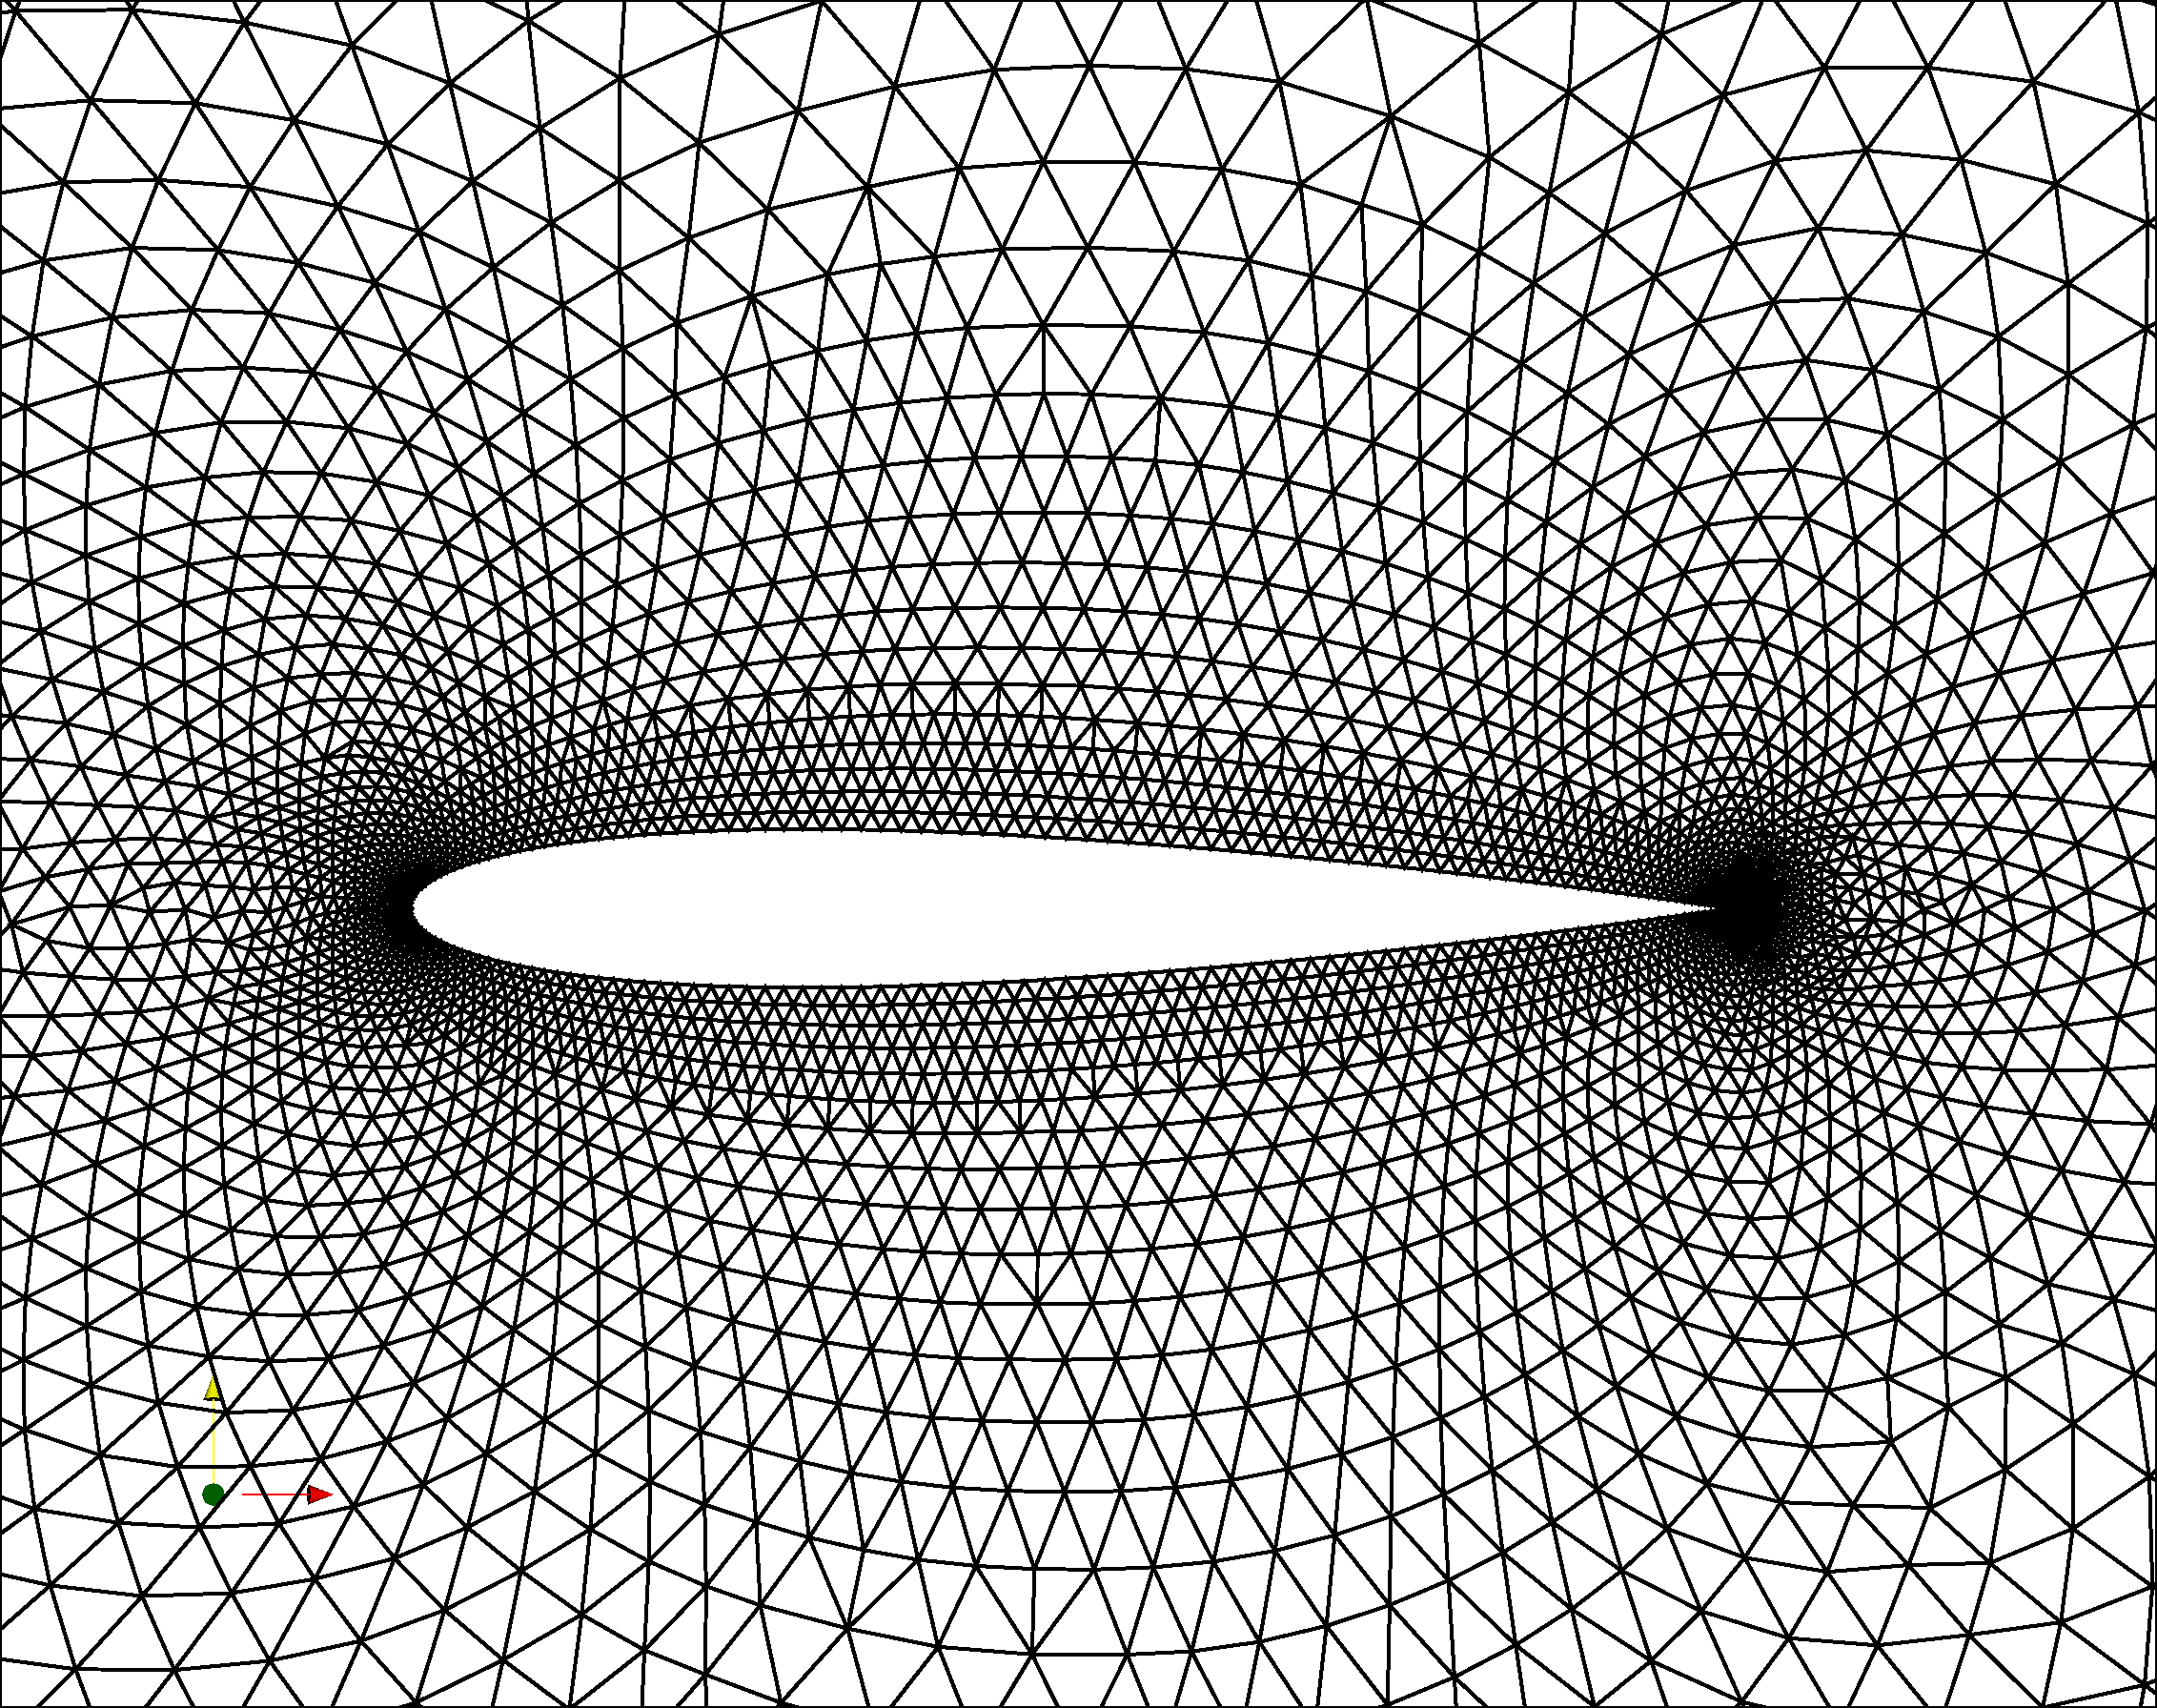
\includegraphics[width=.75\textwidth]{tut01/mesh.pdf}
    \caption{Unstructured mesh around NACA0012.}
    \label{fig:mesh}
\end{figure}
%--------------------------------------------------------------
\subsection{Visualize Pressure Contour}
In order to visualize pressure contour, click on the \textit{flow}.vtk from \textbf{Pipeline Browser} to activate the file, and then click on the \textbf{Properties} tab. According to Fig.\ref{fig:colorby}, in \textbf{Coloring} section, select \textit{Pressure} from drop-down menu. To change color settings for the pressure, you can also click on the \textbf{Edit} under the \textbf{Coloring}. Normally another display window appears on the right-hand side of the monitor, similar to Fig.\ref{fig:change_color_range}. Now you can change the maximum/minimum range of pressure to your desirable values by \textbf{Set Range}, or change contour colors by \textbf{Choose Preset} (Fig.\ref{fig:change_color_range}).
\begin{figure}[htbp]
    \centering
    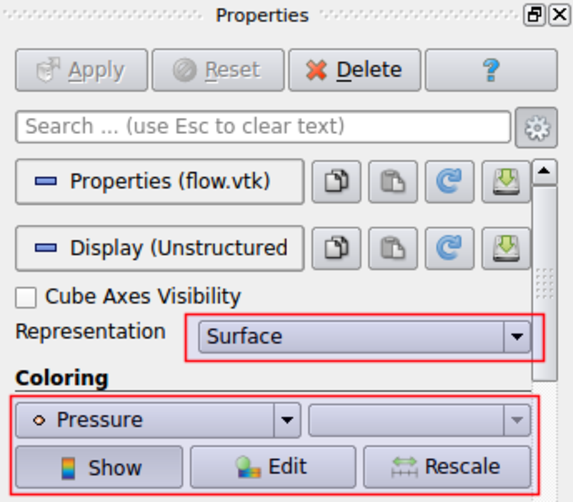
\includegraphics[width=0.4\textwidth]{tut01/contourdisplay.pdf}
    \caption{Contour settings in \textbf{Display} tab.}
    \label{fig:colorby}
\end{figure}
\begin{figure}[htbp]
    \centering
    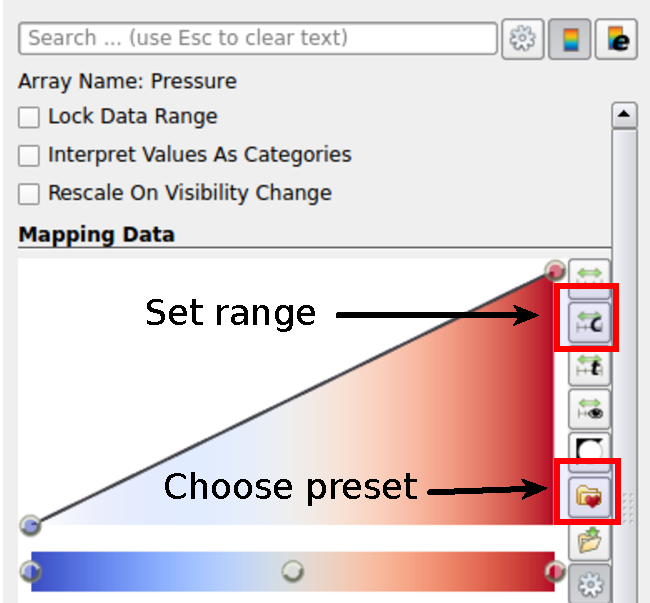
\includegraphics[width=0.5\textwidth]{tut01/colormap.pdf}
    \caption{How to change color and max/min values for contour.}
    \label{fig:change_color_range}
\end{figure}
After taking these steps, the pressure contour in the display window should be similar to Fig.\ref{fig:pressure_contour}.
\begin{figure}[htbp]
    \centering
    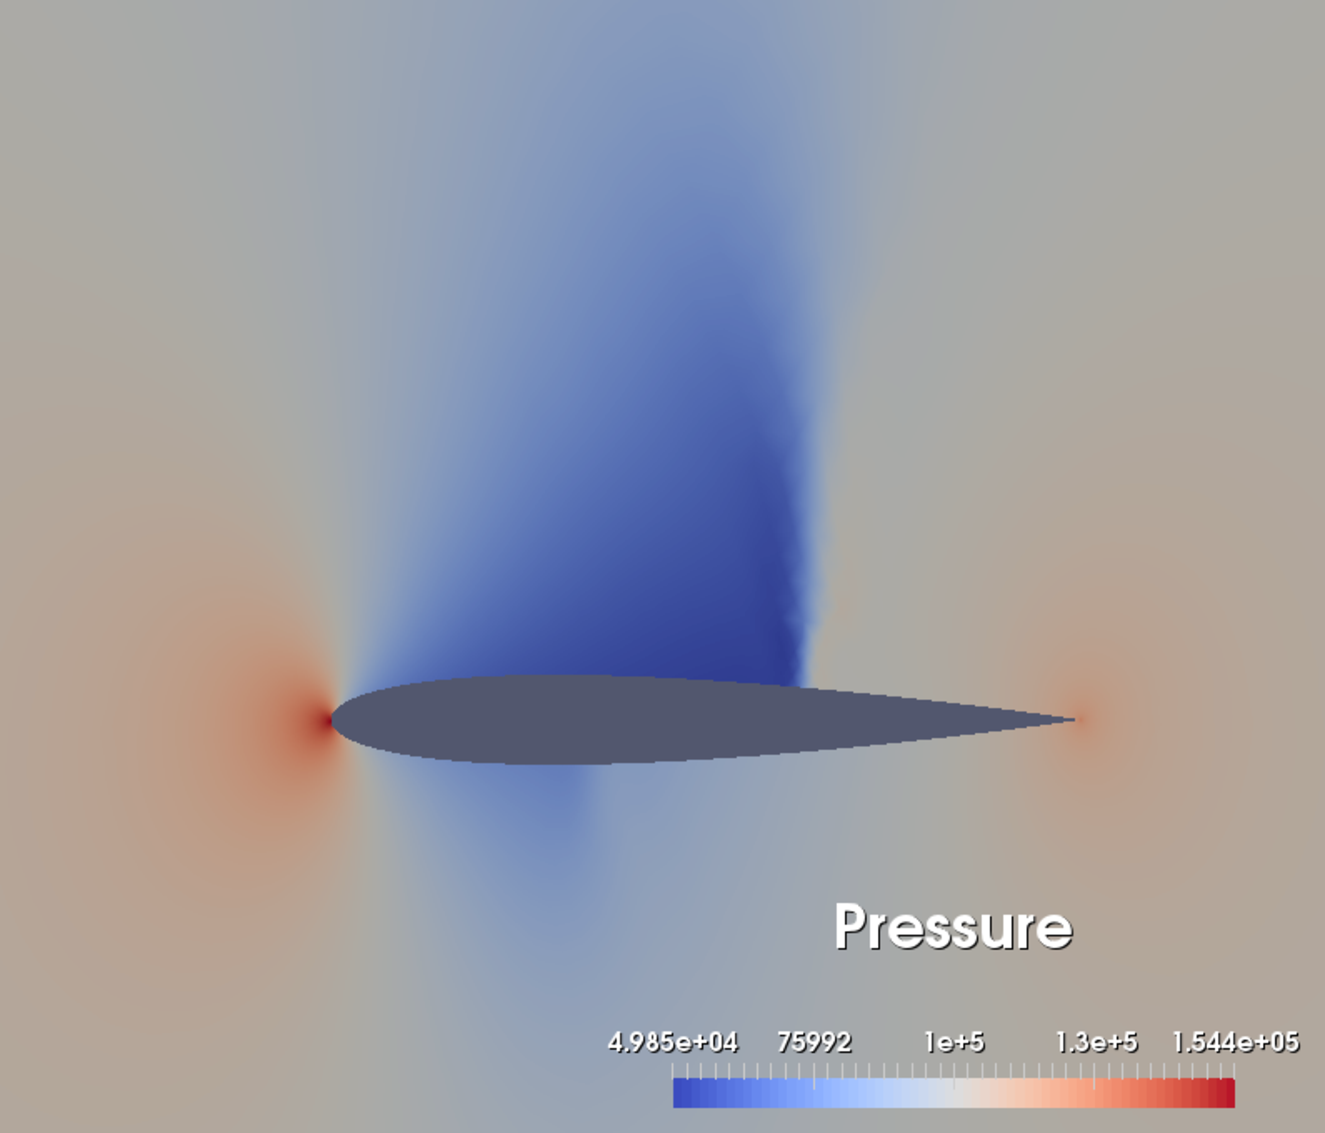
\includegraphics[width=.75\textwidth]{tut01/pressurecontour1.pdf}
    \caption{Pressure contour for NACA0012 airfoil.}
    \label{fig:pressure_contour}
\end{figure}

To add contour lines, click again on the \textit{flow}.vtk file in the \textbf{Pipeline Browser}, and then click on the \textbf{Contour} icon (Fig.\ref{fig:contour_icon}) in toolbar.
\begin{figure}[htbp]
    \centering
    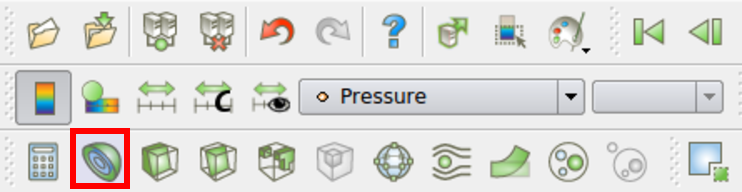
\includegraphics[width=0.6\textwidth]{tut01/contourlineicon.pdf}
    \caption{Contour icon in toolbar.}
    \label{fig:contour_icon}
\end{figure}
Now you should see \textit{Contour1} appears under \textit{flow}.vtk file in the \textbf{Pipeline Browser} (Fig.\ref{fig:contour1}).
\begin{figure}[htbp]
    \centering
    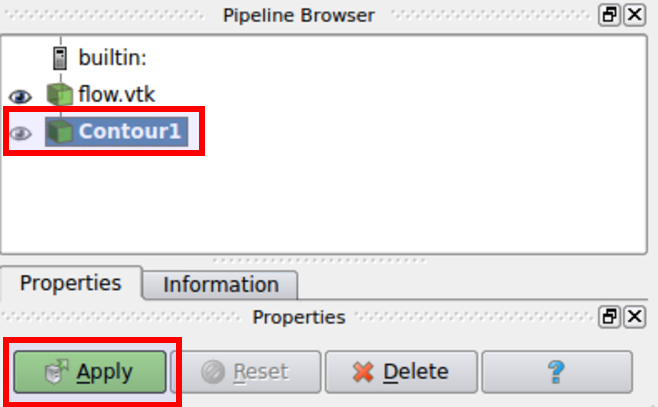
\includegraphics[width=0.5\textwidth]{tut01/contour1.pdf}
    \caption{Adding \textit{Contour1} in \textbf{Pipeline Browser}.}
    \label{fig:contour1}
\end{figure}
According to Fig.\ref{fig:contourby a}, go to the \textbf{Properties} tab, and select \textit{Pressure} from \textbf{Contour By} drop-down menu. Next, click on the \textbf{New Range} icon to customize the range of pressure contour. For now, set the number of step to 20, similar to Fig.\ref{fig:contourby b}. It means the pressure contour range is equally divided by 20 portions, and the pressure values in each portion are limited by two lines in the display window. At the end, click on \textbf{Apply} to see contour lines in display window.
\begin{figure}[htbp]
    \centering
     \begin{subfigure}[b]{.4\textwidth}
         \centering
         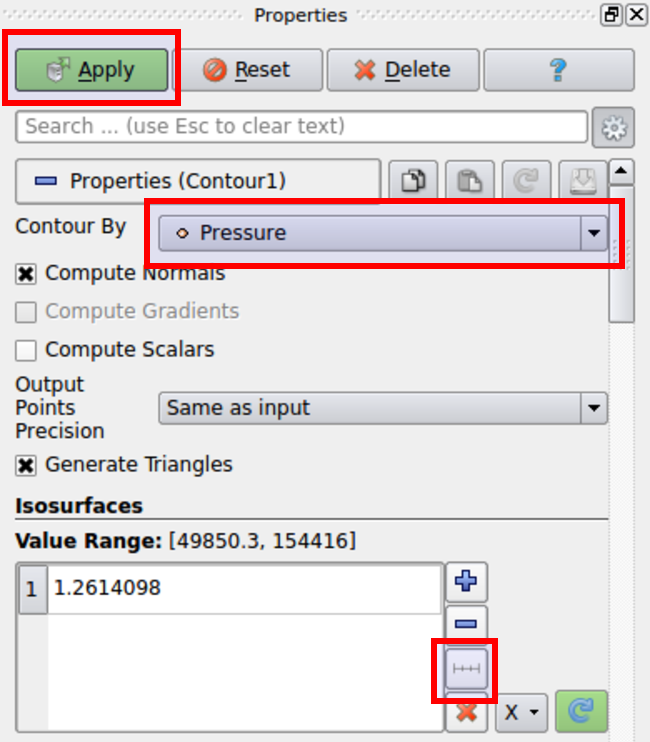
\includegraphics[width=1.0\textwidth]{tut01/contourlinenewrange.pdf}
         \caption{Define new range}
         \label{fig:contourby a}
     \end{subfigure}
     \hfill
     \begin{subfigure}[b]{.4\textwidth}
         \centering
         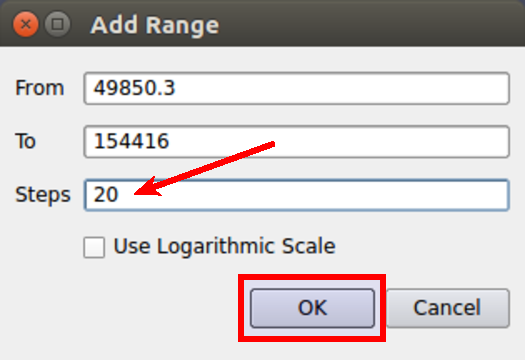
\includegraphics[width=1.0\textwidth]{tut01/addrangepdf.pdf}
         \caption{Add range}
         \label{fig:contourby b}
     \end{subfigure}     
    \caption{How to define a new range for the contour lines.}
    \label{fig:contourby}
\end{figure}
Next, as it is shown in Fig.\ref{fig:colorby2}, click on the \textbf{Display} under \textbf{Properties} tab. In \textbf{Coloring} section, select \textbf{Solid Color} form drop-down menu, and choose white color form \textbf{Edit}.
\begin{figure}[htbp]
    \centering
    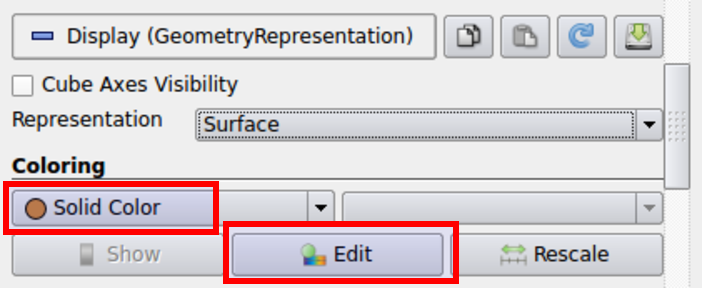
\includegraphics[width=0.6\textwidth]{tut01/coloring.pdf}
    \caption{Changing contour lines color in \textbf{Coloring} section.}
    \label{fig:colorby2}
\end{figure}
Eventually, the pressure contour with contour lines should be similar to Fig.\ref{fig:pressure_contour_lines}.
\begin{figure}[htbp]
    \centering
    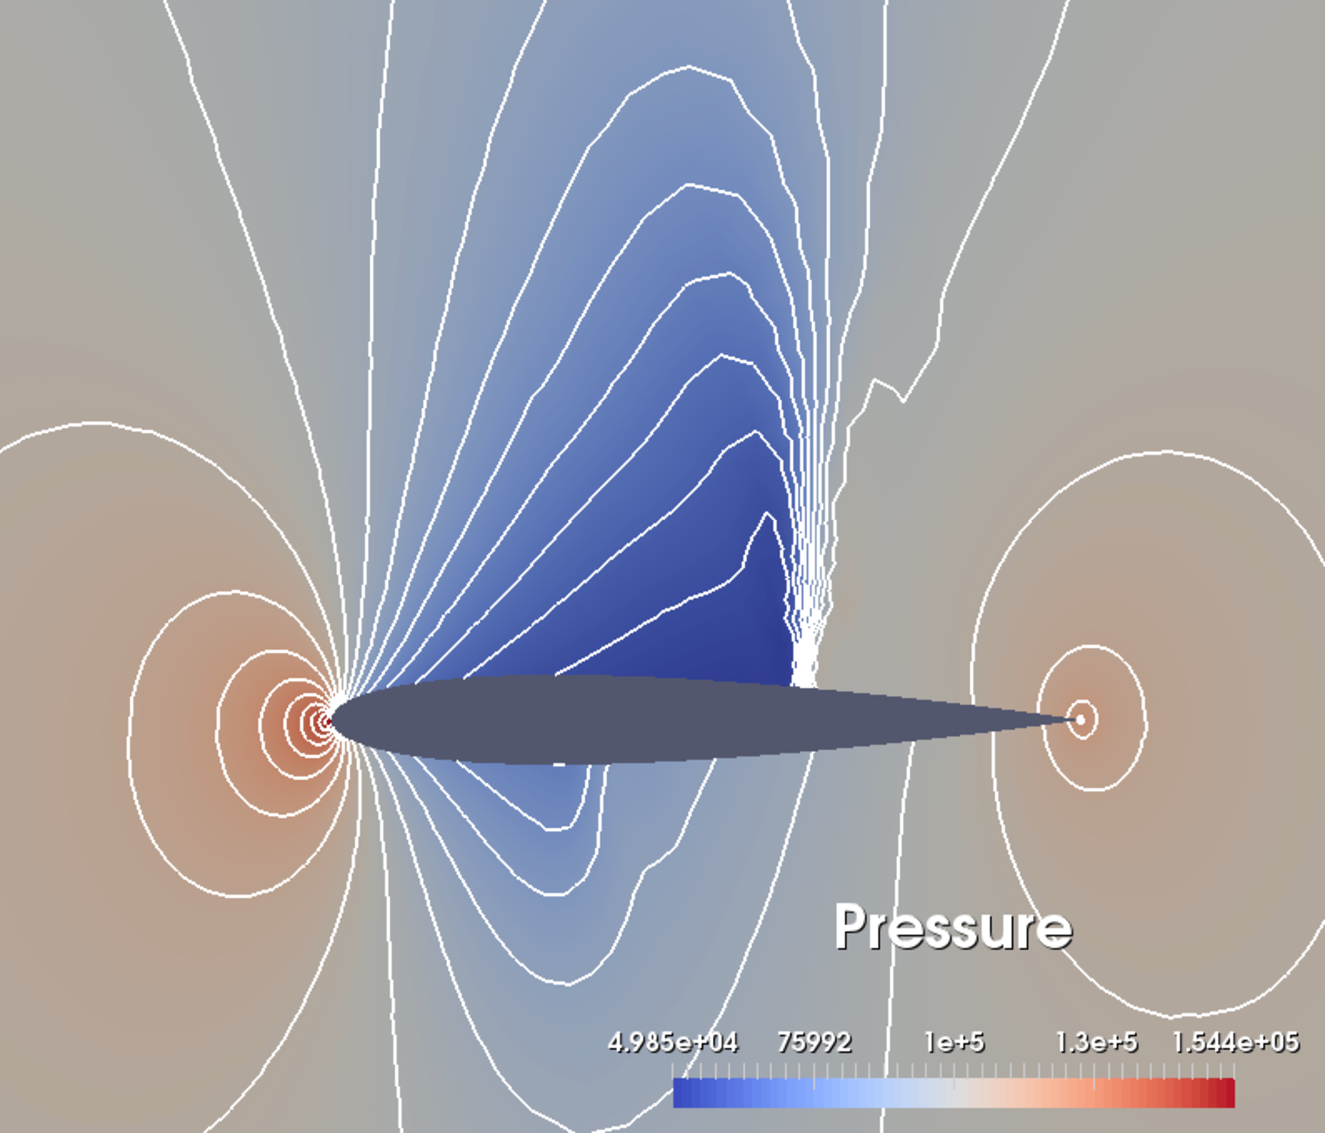
\includegraphics[width=.75\textwidth]{tut01/pressurecontour2.pdf}
    \caption{Pressure contour superimposed by contour lines around NACA0012.}
    \label{fig:pressure_contour_lines}
\end{figure}
%--------------------------------------------------------------
\subsection{Visualize Pressure Coefficient}
The pressure data on the surface of the airfoil is stored in \textit{surface\_flow}.vtk. Now the attempt is to plot it with respect to the chord line position. Therefore, go to \textbf{Open} $\rightarrow$ \textbf{File}, and select \textit{surface\_flow}.vtk. As it is shown in Fig.\ref{fig:builtin}, this file is now loaded and added to the list of items under \textbf{builtin} in \textbf{Pipeline Browser}.
\begin{figure}[htbp]
    \centering
    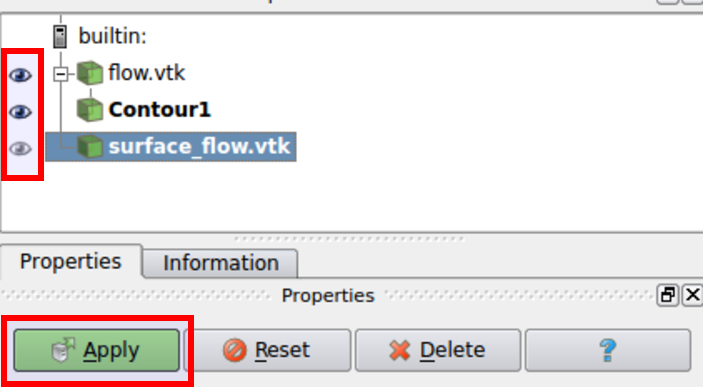
\includegraphics[width=0.5\textwidth]{tut01/eyeiconsurfaceflow.pdf}
    \caption{Loading another .vtk file in Paraview.}
    \label{fig:builtin}
\end{figure}
Note that there is an eye icon on the left-hand side of each item in \textbf{Pipeline Browser}, which enables to hide/unhide the figures being related to each item. Since we want to see pressure coefficient plot, we hide the contours by clicking on the eye icon beside \textit{flow}.vtk and \textit{Contour1}. 

According to Fig.\ref{fig:plotdata}, select \textit{surface\_flow}.vtk in \textbf{Pipeline Browser}, and then go to \textbf{Filters} $\rightarrow$ \textbf{Search} (Fig.\ref{fig:plotdata a}), and then search for \textbf{Plot Data} (Fig.\ref{fig:plotdata b}). 
\begin{figure}[htbp]
    \centering
     \begin{subfigure}[b]{.4\textwidth}
         \centering
         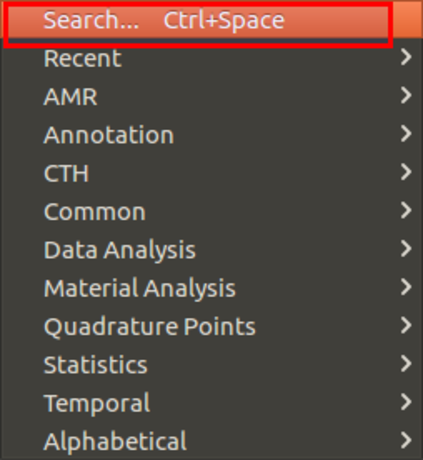
\includegraphics[width=1.0\textwidth]{tut01/filtersearch.pdf}
         \caption{Search item in \textbf{Filter}}
         \label{fig:plotdata a}
     \end{subfigure}
     \hfill
     \begin{subfigure}[b]{.4\textwidth}
         \centering
         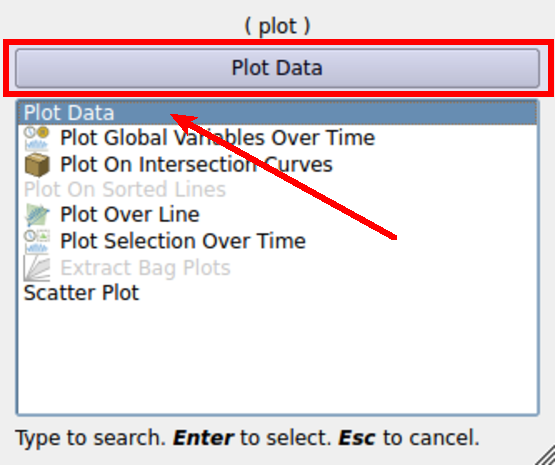
\includegraphics[width=1.0\textwidth]{tut01/plotdatasearch.pdf}
         \caption{Searching for \textbf{PotData}}
         \label{fig:plotdata b}
     \end{subfigure}     
    \caption{How to plot data.}
    \label{fig:plotdata}
\end{figure}

After taking this step, as it is shown in Fig.\ref{fig:plotdata-list}, \textit{PlotData1} item is added to the list in the \textbf{Pipeline Browser}. Then, hide (deactivate) all items in the list of \textbf{Pipeline Browser} except \textit{PlotData1} by clicking on the eye icons beside each item, and later, click on \textbf{Apply} for the next step.
\begin{figure}[htbp]
    \centering
    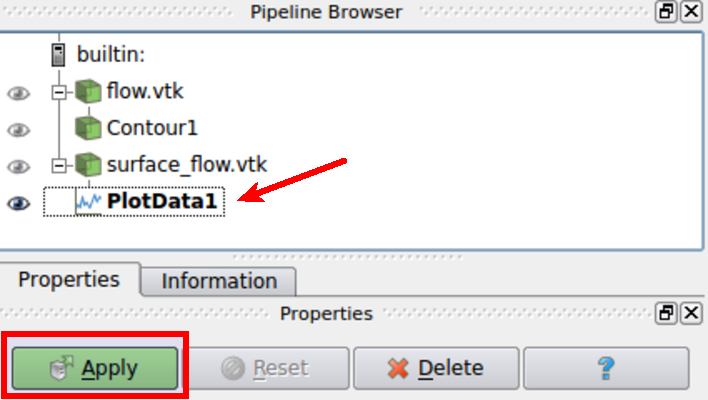
\includegraphics[width=0.5\textwidth]{tut01/plotdata1.pdf}
    \caption{Adding \textit{PlotData1} to \textbf{Pipeline Browser}.}
    \label{fig:plotdata-list}
\end{figure}
According to Fig.\ref{fig:pointsx}, from \textbf{Display} in \textbf{Properties} tab, deactivate \textbf{Use Index For XAxis}, and then select \textit{Points\_X} from drop-down menu. 
\begin{figure}[htbp]
    \centering
    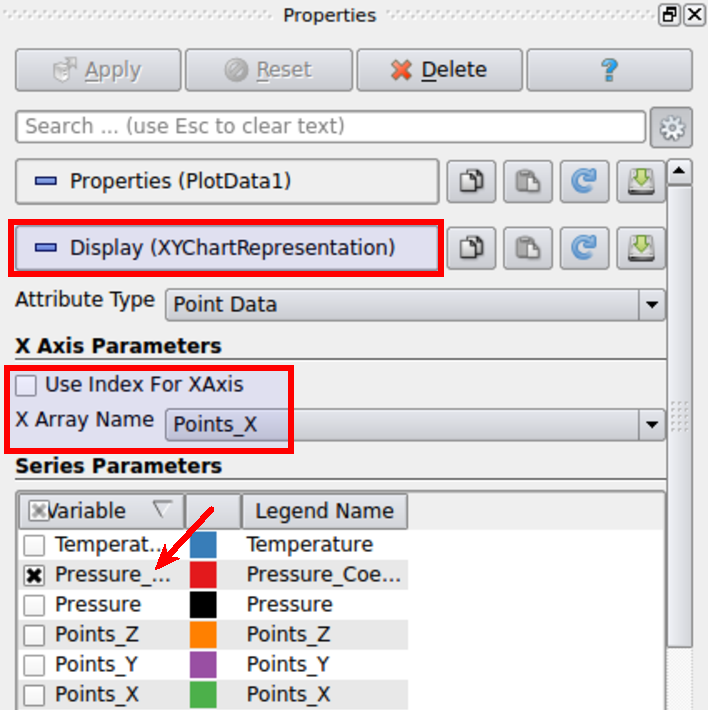
\includegraphics[width=0.5\textwidth]{tut01/plotcurvesetting.pdf}
    \caption{Plot settings for pressure coefficient along the chord line.}
    \label{fig:pointsx}
\end{figure}
In the \textbf{Series Parameters} in the same tab, unclick all variables except for \textit{Pressure\_Coefficient}. This allows you to have only one plot for pressure coefficient versus chord line. The pressure plot in the display window should be similar to Fig.\ref{fig:surface_pressure}.
\begin{figure}[htbp]
    \centering
    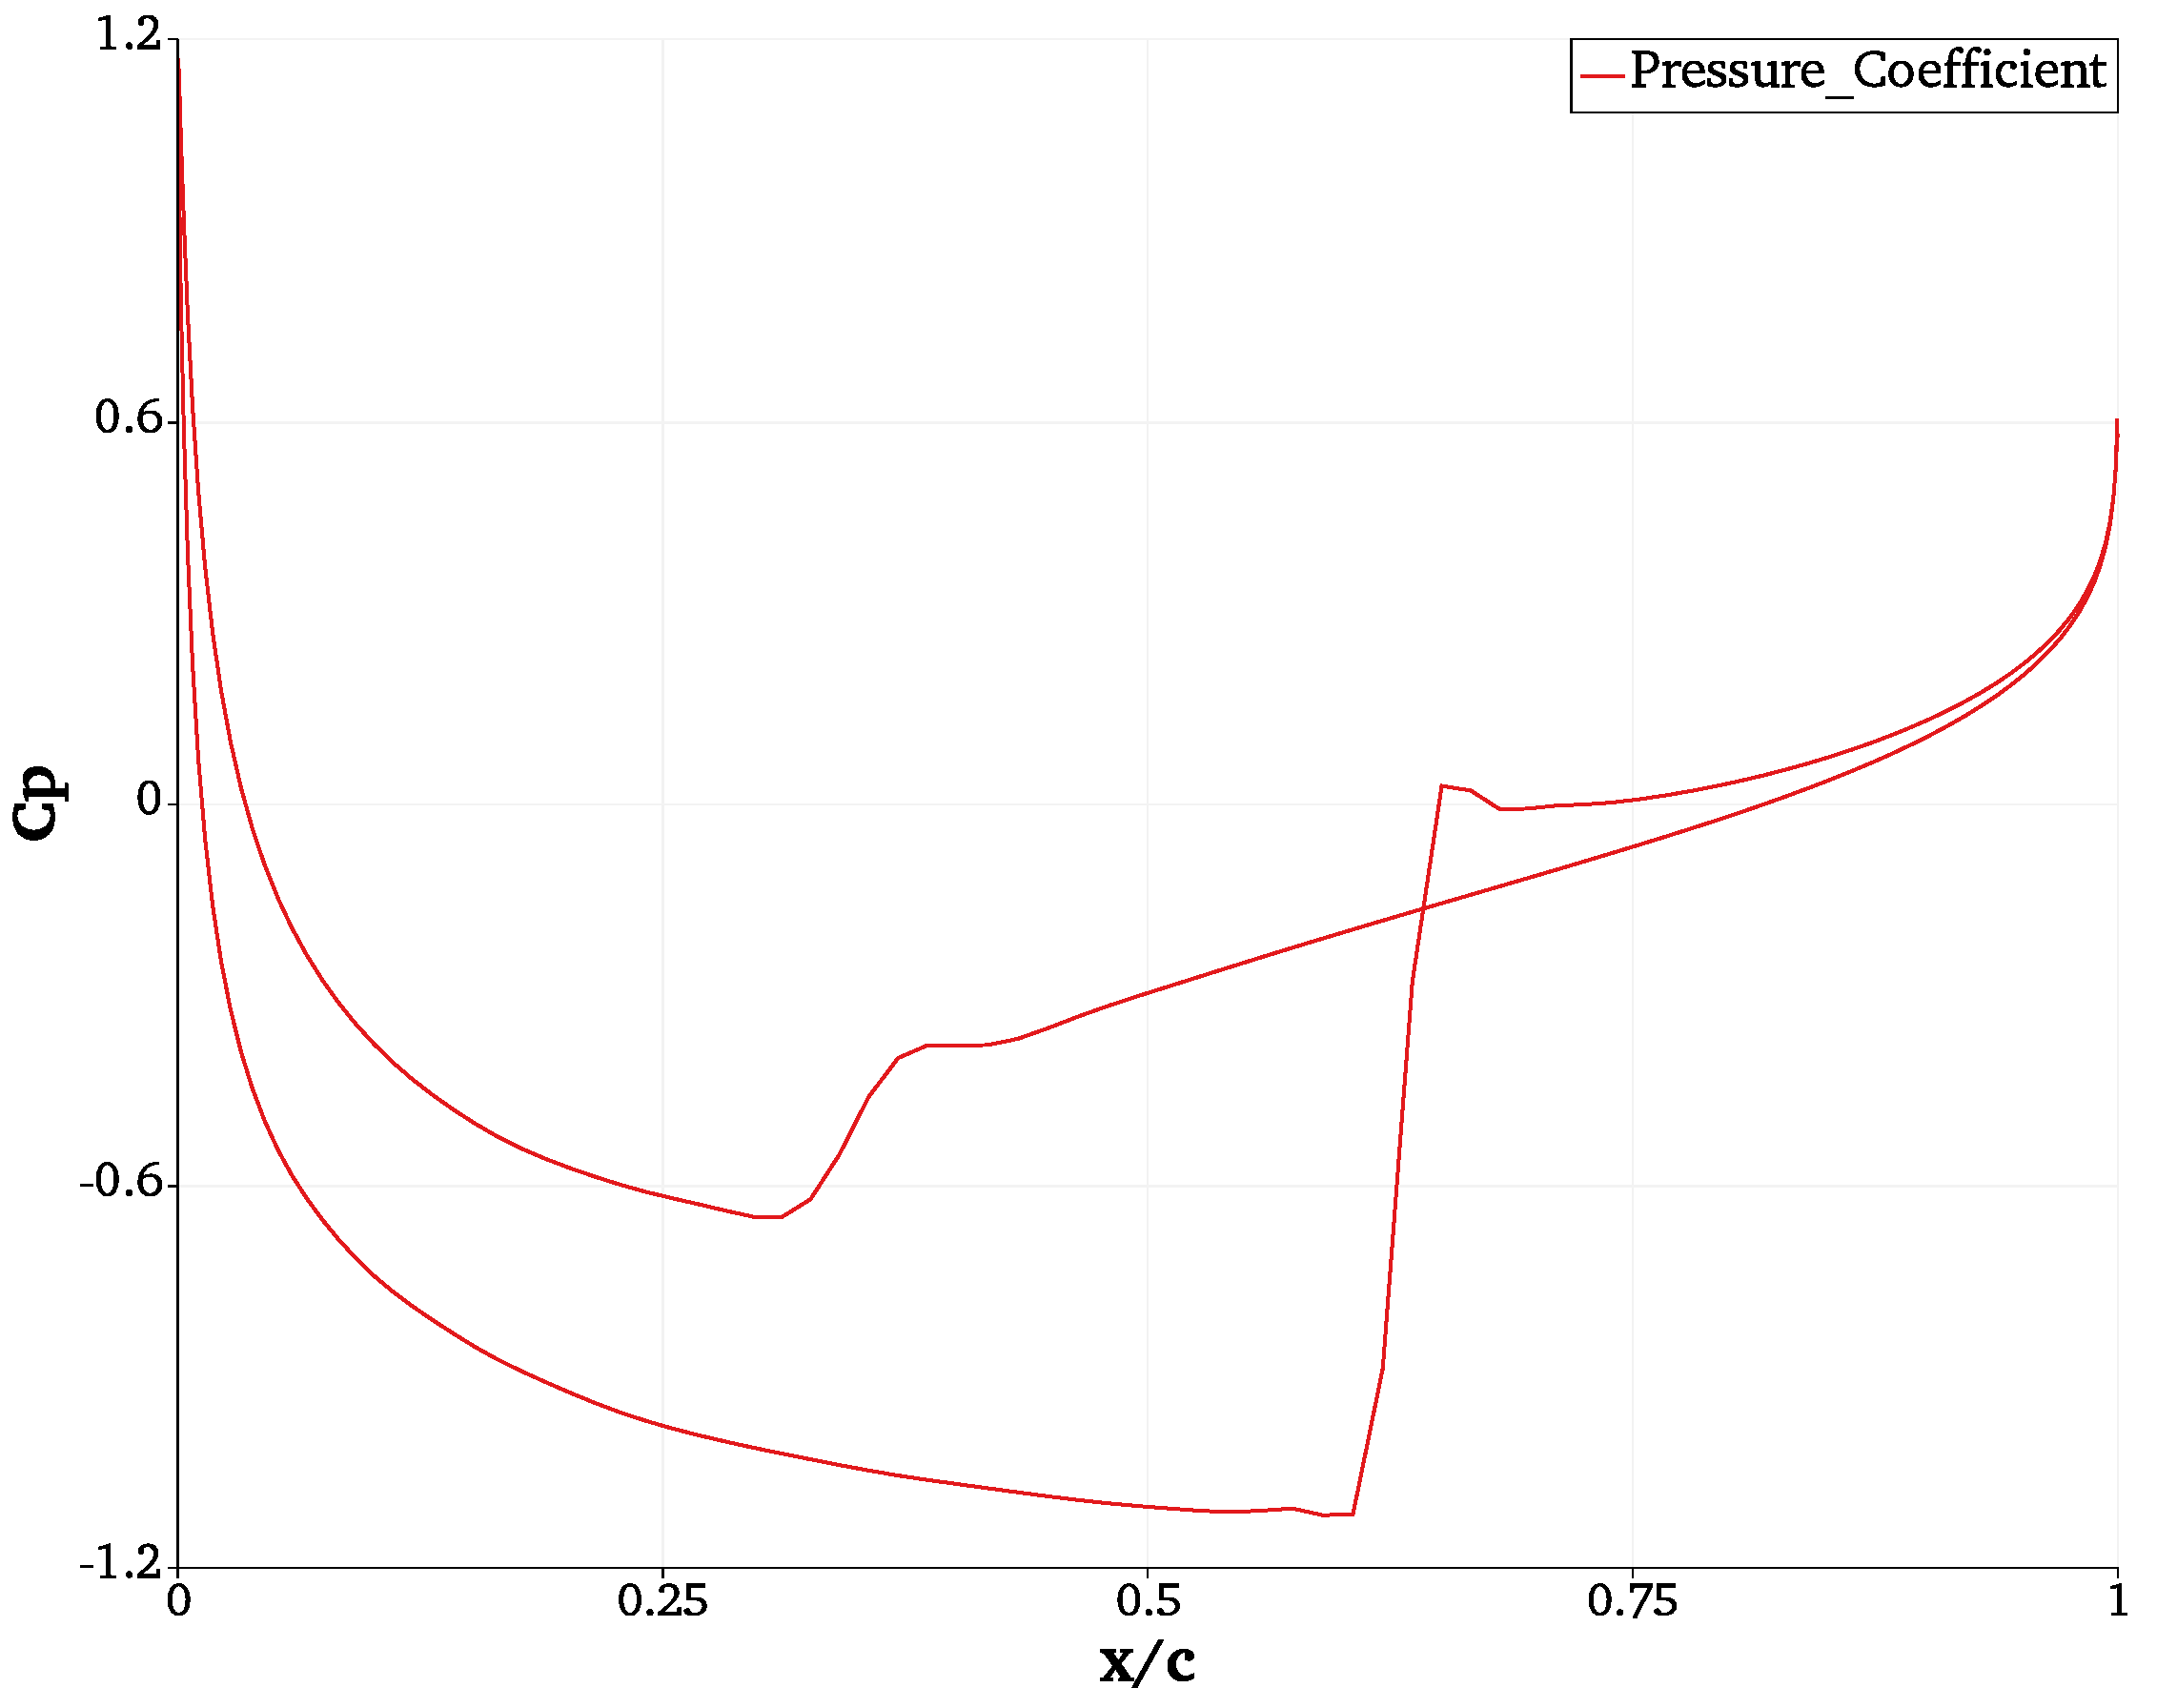
\includegraphics[width=.75\textwidth]{tut01/plot11.pdf}
    \caption{Pressure coefficient on the surface of the NACA0012.}
    \label{fig:surface_pressure}
\end{figure}

Usually $C_p$ is plotted in such a way that the pressure curve in suction side (lower pressure) is on top of the pressure curve on the pressure side (higher pressure). Therefore, we need to reverse  the $y$-axis in the plot (flip). To do this, go to \textbf{Display} from \textbf{Properties} tab. Next, find \textbf{Left Axis Range} section in the same tab, and then click on the \textbf{Left Axis Use Custom Range} (Fig.\ref{fig:viewsetting}). Later, another section appears to select maximum/minimum ranges for left axis of plot. Eventually, just switch numbers in these two text bars. It allows the $y$-axis to be reverse (flipped) as we want it to be.
\begin{figure}[htbp]
    \centering
    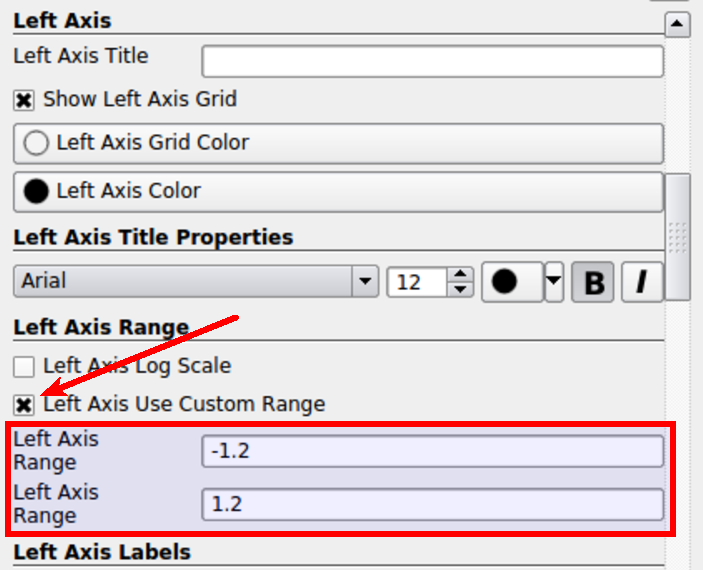
\includegraphics[width=0.5\textwidth]{tut01/leftaxis.pdf}
    \caption{Plot Settings.}
    \label{fig:viewsetting}
\end{figure}
Additionally, there are other parameters that you might change in the same tab, like \textbf{Left Axis Title} or  \textbf{Bottom Axis Title}. To do this, please type $C_p$ and $x/c$ in \textbf{Left Axis Title} and \textbf{Bottom Axis Title}, respectively. Furthermore, for adding marker to the plot lines, form \textbf{Display} select \textbf{Marker Style} as \textit{Diamond} (Fig.\ref{fig:marker}). You can also change the thickness of plot line in the same tab.
\begin{figure}[htbp]
    \centering
    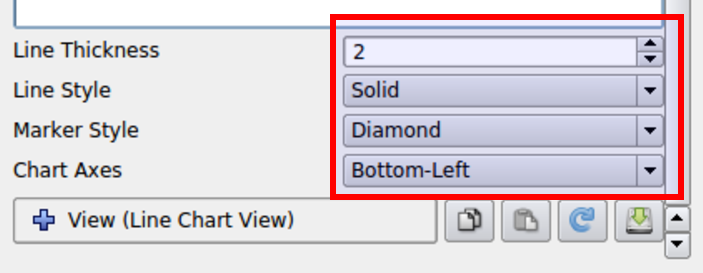
\includegraphics[width=0.4\textwidth]{tut01/addingmarker.pdf}
    \caption{How to add marker to plot.}
    \label{fig:marker}
\end{figure}
Eventually, the final plot you should get is like Fig.\ref{fig:surface_pressure2}
\begin{figure}[htbp]
    \centering
    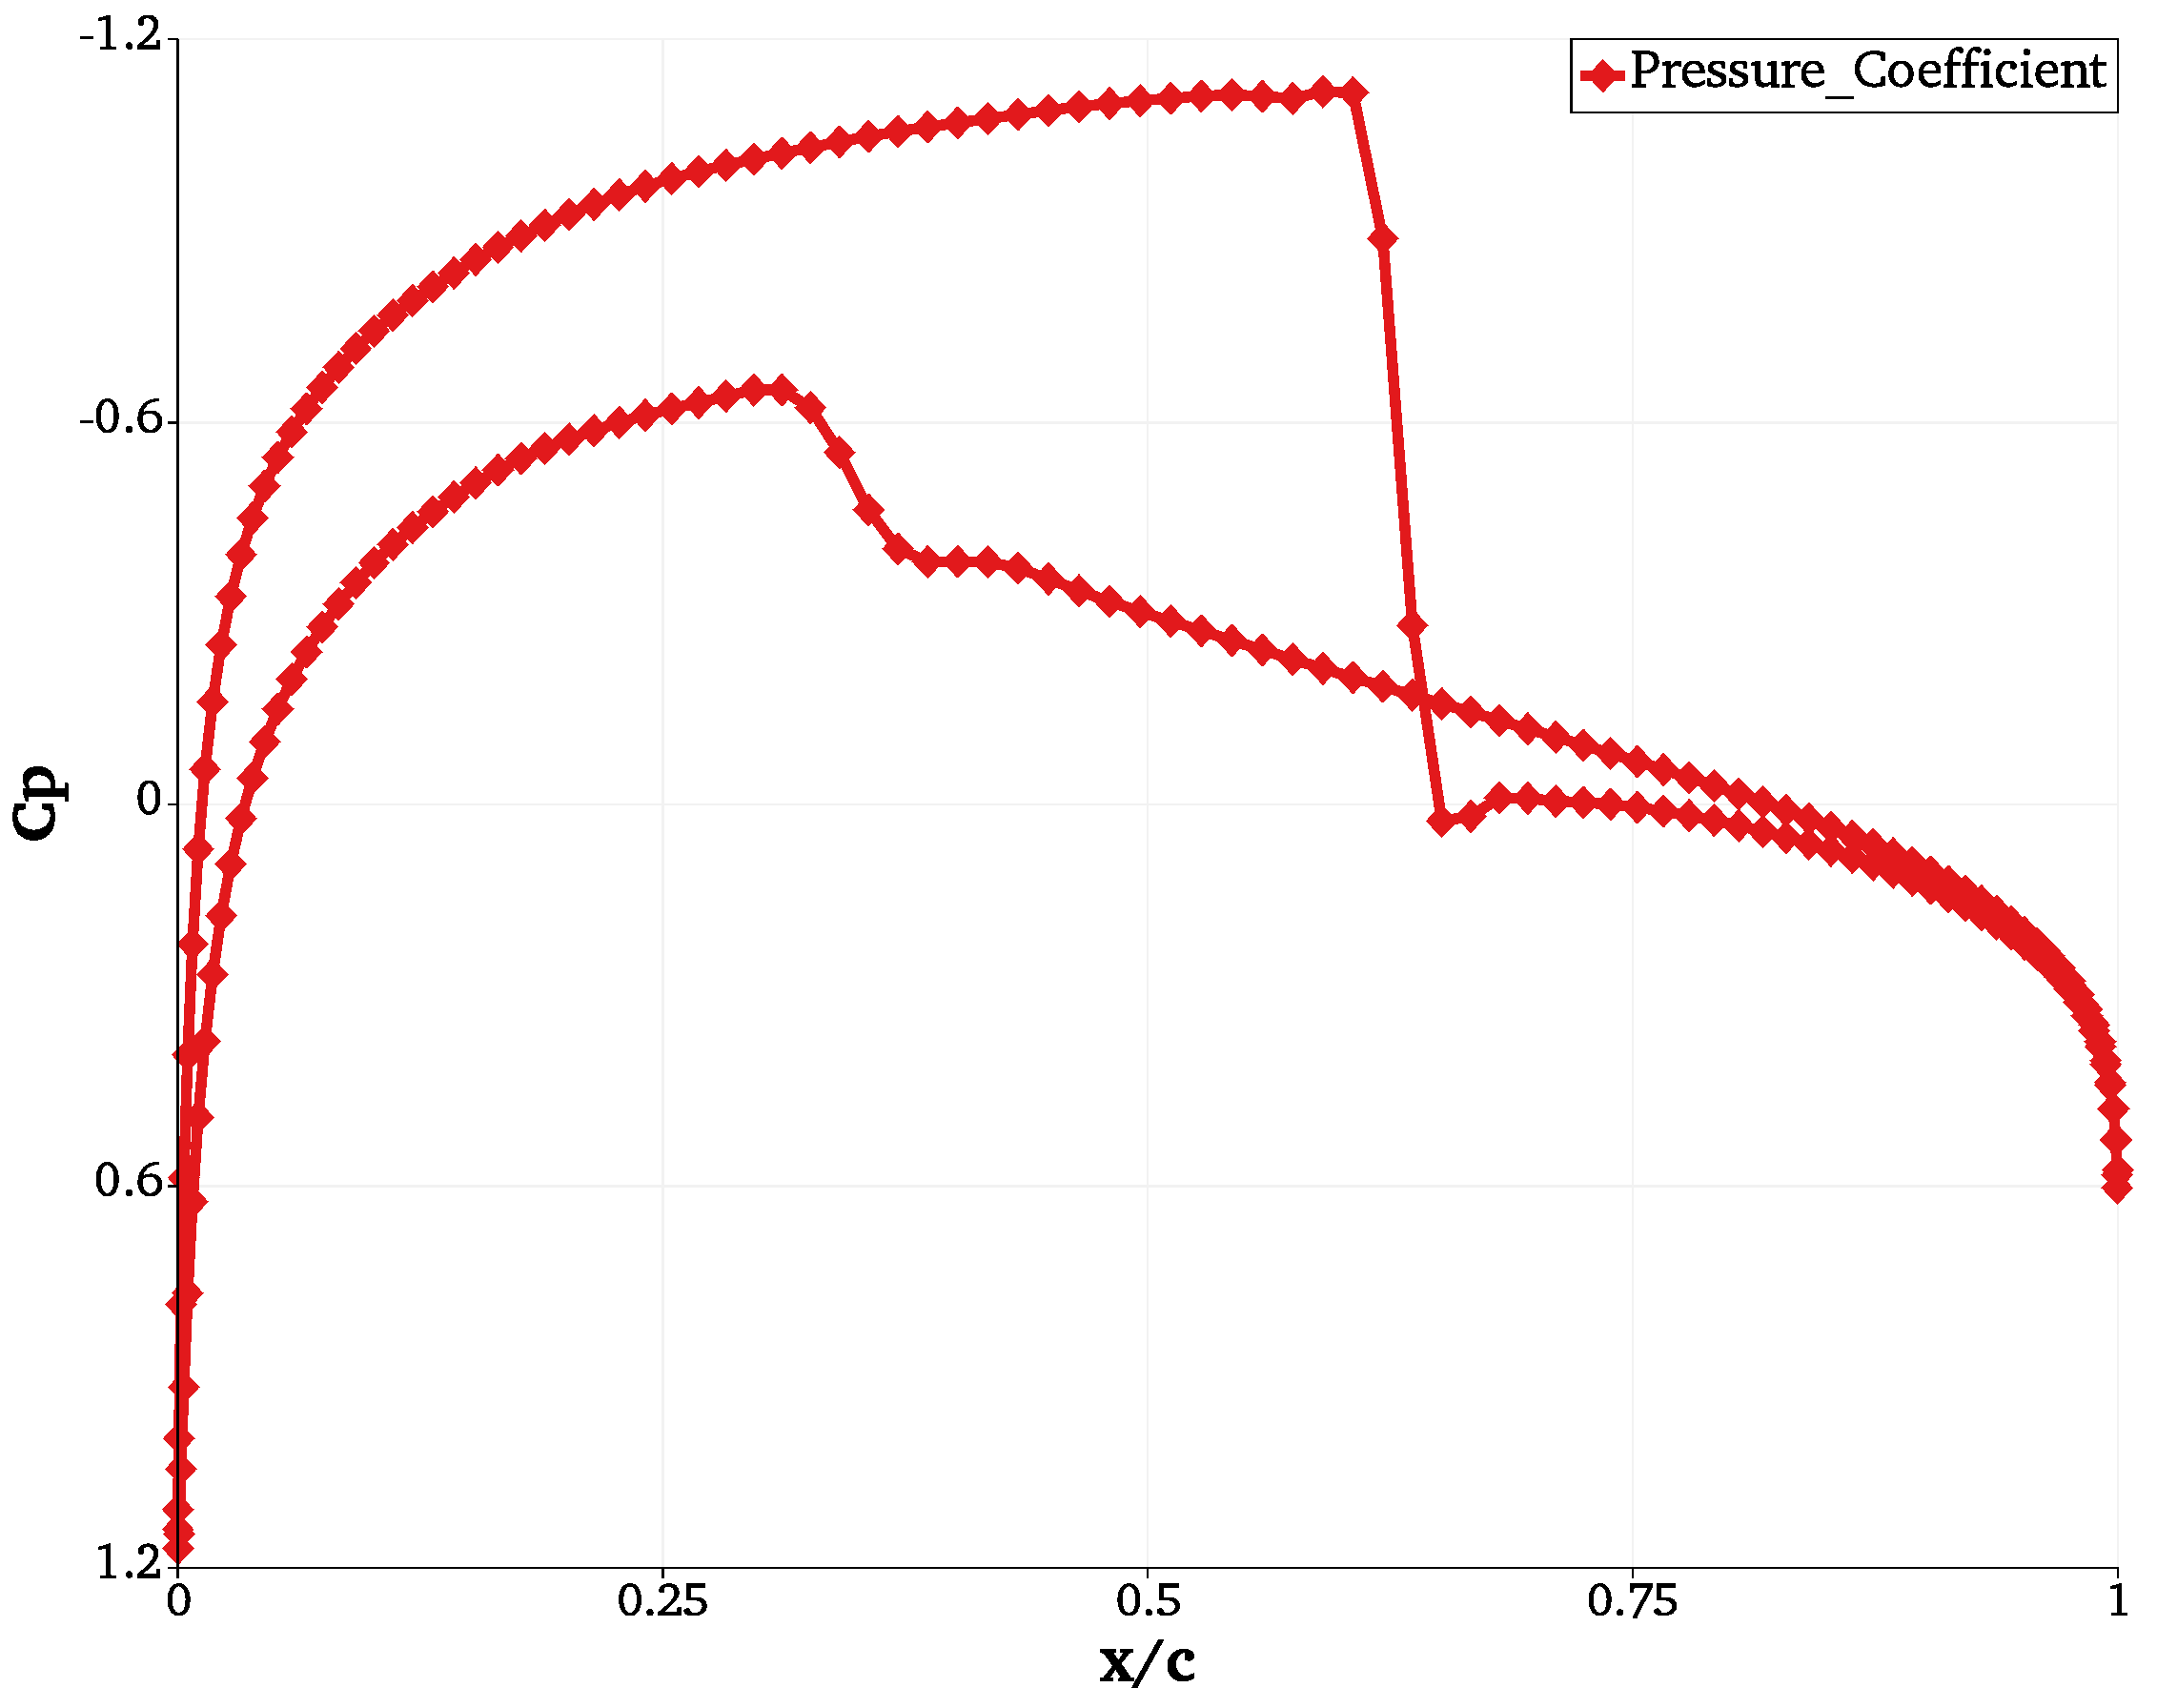
\includegraphics[width=.75\textwidth]{tut01/plot22.pdf}
    \caption{Revised version of the pressure coefficient plot on the surface of the NACA0012.}
    \label{fig:surface_pressure2}
\end{figure}
%--------------------------------------------------------------
\subsection{Forces on the Airfoil}
In order to obtain the aerodynamic loads on the airfoil, open \textit{force\_breakdown}.dat using a text editor software. According to Fig.\ref{fig:forcefile1}, in this file there are flow properties that you can check if the values are the same as those in configuration file. 
\begin{figure}[htbp]
    \centering
    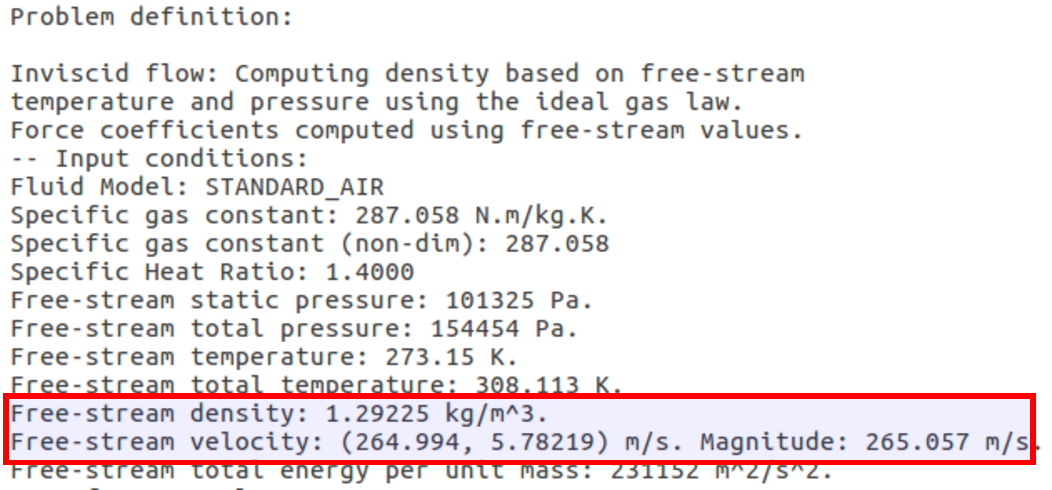
\includegraphics[width=0.9\textwidth]{tut01/forcefile1.pdf}
    \caption{Fluid and flow properties form \textit{force\_breakdown}.dat.}
    \label{fig:forcefile1}
\end{figure}

Additionally, according to Fig.\ref{fig:forcefile2}, the aerodynamic loads are expressed in non-dimensional form by using free-stream values for density and velocity, as well as one reference length (or area). It could be a good practice to check if the non-dimensional factor corresponds to the expected free-stream values. The actual forces (dimensional) can be obtained by multiplying coefficient with non-dimensional factor calculated by free-stream density and velocity. Note that you can find lift coefficient ($C_L$), drag coefficient ($C_D$), lift to drag ratio ($C_L / C_D$), the moment coefficient ($C_{M,z}$), $x$-component of force coefficient ($C_{F,x}$) and $y$-component of force coefficient ($C_{F,y}$) all from the \textit{force\_breakdown}.dat.
\begin{figure}[htbp]
    \centering
    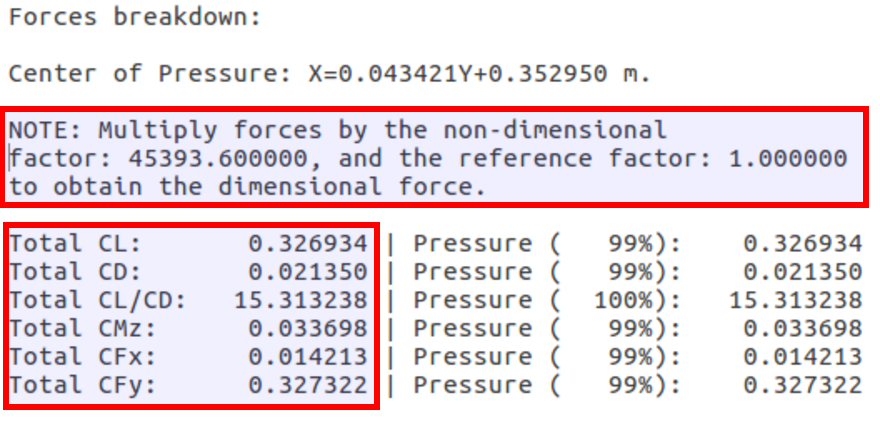
\includegraphics[width=0.8\textwidth]{tut01/forcefile2.pdf}
    \caption{Aerodynamic loads from \textit{force\_breakdown}.dat.}
    \label{fig:forcefile2}
\end{figure}

%++++++++++++++++++++++++++++++++++++++++++++++++++++++++++++++
\section{Questions}
1. Run the provided default NACA0012 test case at the provided Ma = 0.8.
\begin{enumerate}[label=(\alph*)]
    \item Plot and comment on the mesh.
    \item Plot and comment on the pressure contours around the airfoil.
    \item Plot and comment on the pressure coefficient on the surface of the airfoil.
\end{enumerate}
2. Re-run the default NACA0012 case but change the Mach number to Ma = 0.3 and run several simulations using alpha = 0, 2, 4, 6, 8, 10, 12, 14, 16 degrees.
\begin{enumerate}[label=(\alph*)]
    \item Plots Cl vs alpha alongside the provided experimental data \cite{ladson1988effects} in the test case folder.
    \item Repeat 1.b with Ma = 0.3 for the alpha = 0, 8, 16 degree cases.
    \item Repeat 1.c with for the alpha = 0, 8, 16 degree cases and include the provided experimental data  in the \cite{ladson1987pressure}.
\end{enumerate}
3. Compare your CFD results in Question 2). Discuss sources of error that could have led to any discrepancies in your results.
%--------------------------------------------------------------
%++++++++++++++++++++++++++++++++++++++++++++++++++++++++++++++
\chapter{Supersonic Wedge}

\chapter{Inviscid ONERA M6}

\chapter{Laminar Flat Plate}

\chapter{Laminar Cylinder}

\chapter{Turbulent ONERA M6}
